\part{VLSI Experiments}
\chapter{Digital Experiments}
\section{Combinational Circuits}

\subsection{Full Adder}

\subsection*{Aim}

To design and synthesize  a full adder using  verilog and verify its functionality using RTL and Gate Level Simulation and to draw its layout.  Also find the area consumed, power and delay of the full adder.

\subsection*{Program}
\subsubsection*{Full Adder Source}
\begin{Verbatim}

/***************************************************************************
				FULL ADDER	
***************************************************************************/
`timescale 1ns / 1ps
module full_adder(x,y,cin,sum,cout);

	input x,y,cin;
	output sum,cout;
	
	assign sum=(x^y)^cin;
	assign cout=(x&y)|(x&cin)|(y&cin);
	
endmodule

\end{Verbatim}
\pagebreak


\paragraph{Full Adder Testbench}

\begin{Verbatim}
/***************************************************************************
				FULL ADDER - TESTBENCH
***************************************************************************/
`timescale 1ns / 1ps
module full_adder_tb;

	// Inputs
	reg x;
	reg y;
	reg cin;

	// Outputs
	wire sum;
	wire cout;

	// Instantiate the Unit Under Test (UUT)
	full_adder uut (
		.x(x), 
		.y(y), 
		.cin(cin), 
		.sum(sum), 
		.cout(cout)
	);

	initial begin
		// Initialize Inputs
		
		//Case 0 : 0+0 with carry in of 0
		x = 0;
		y = 0;
		cin = 0;

		// Wait 100 ns for global reset to finish
		#100;
        
		// Add stimulus here
		
		//Case 0 : 0+0 with carry in of 1
		x = 0;
		y = 0;
		cin = 1;
		#20; 
		
		//Case 0 : 0+1 with carry in of 0
		x = 0;
		y = 1;
		cin = 0;
		#20;
		
		//Case 0 : 0+1 with carry in of 1
		x = 0;
		y = 1;
		cin = 1;
		#20;
		
		//Case 0 : 1+0 with carry in of 0
		x = 1;
		y = 0;
		cin = 0;
		#20;
		
		//Case 0 : 1+0 with carry in of 1
		x = 1;
		y = 0;
		cin = 1;
		#20;
		
		//Case 0 : 1+1 with carry in of 0
		x = 1;
		y = 1;
		cin = 0;
		#20;
		
		//Case 0 : 1+1 with carry in of 1
		x = 1;
		y = 1;
		cin = 1;
		#20;
	
	end
      
endmodule
\end{Verbatim}


\subsection*{Outputs}

\subsubsection*{RTL Simulation}
\FloatBarrier
\begin{figure}[!hp]
\centering
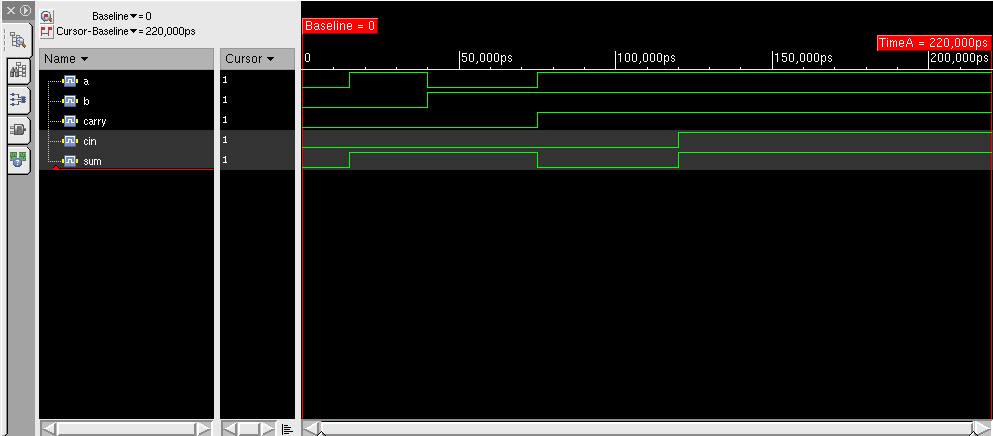
\includegraphics[width=0.9\textwidth]{images/rtl.png}
\caption{RTL Simulation of Full Adder}
\end{figure}

\pagebreak

\subsubsection*{Synthesized Top Level Schematic}
\FloatBarrier
\begin{figure}[!hp]
\centering
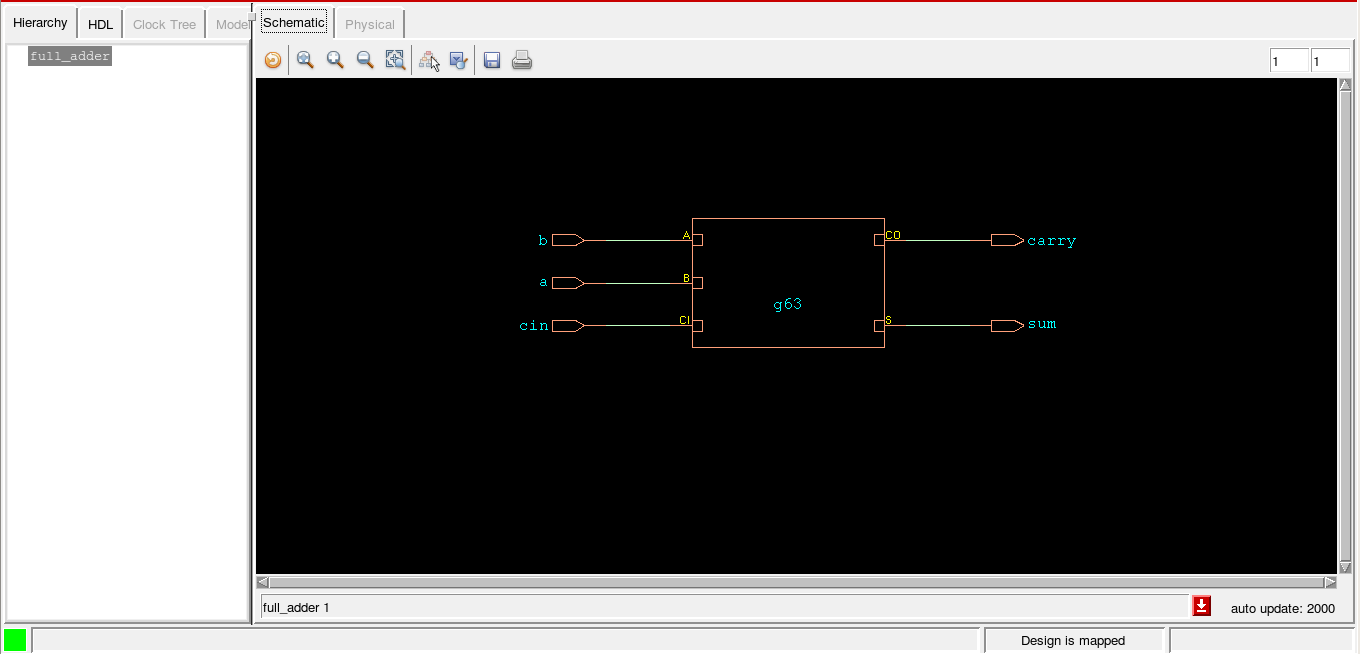
\includegraphics[width=0.9\textwidth]{images/toplevel.png}
\caption{Synthesized Top Level Schematic of Full Adder}
\end{figure}

\subsubsection*{Total Area consumed}
\FloatBarrier
\begin{figure}[!hp]
\centering
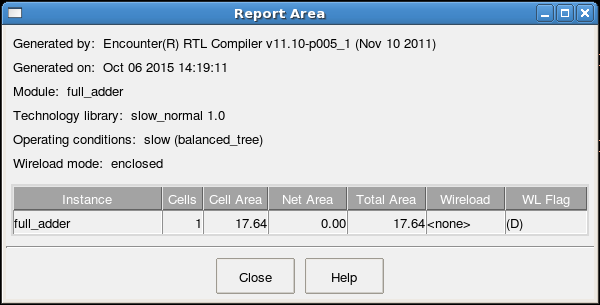
\includegraphics[width=0.9\textwidth]{images/area.png}
\caption{Total Area consumed by Full Adder}
\end{figure}
\pagebreak

\subsubsection*{Total Area consumed}
\FloatBarrier
\begin{figure}[!htpb]
\centering
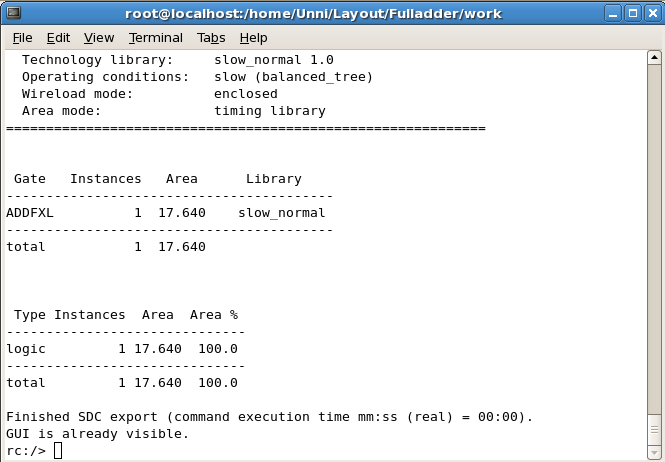
\includegraphics[width=0.8\textwidth]{images/areartl.png}
\caption{Total Area consumed by Full Adder shown in Terminal}
\end{figure}

\subsubsection*{Worst Path Delay}
\FloatBarrier
\begin{figure}[!htpb]
\centering
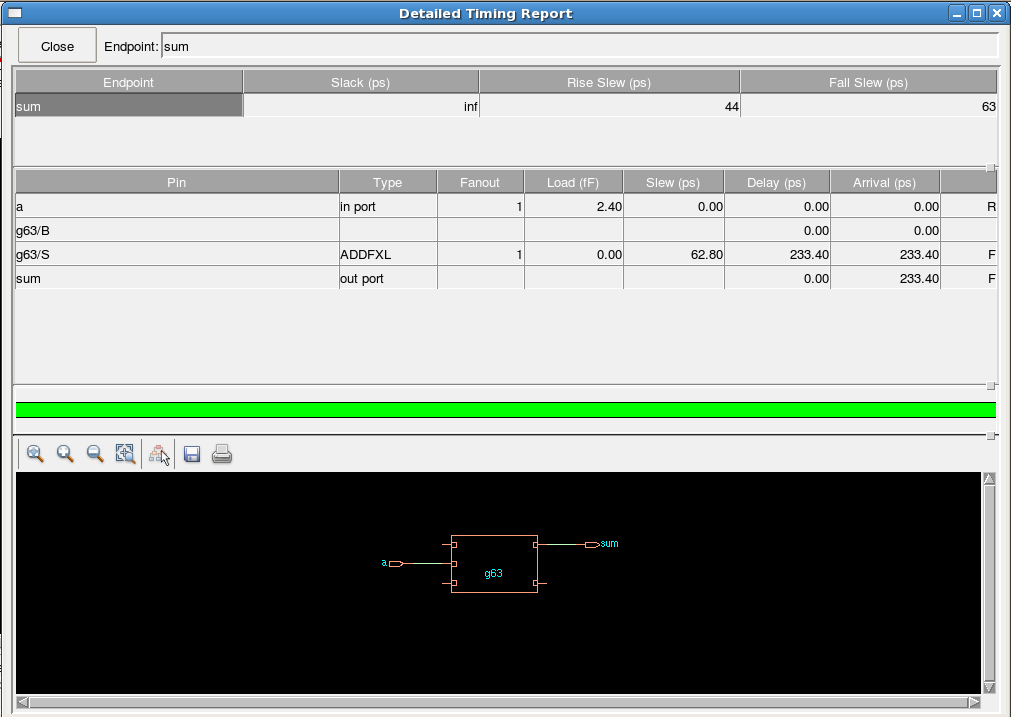
\includegraphics[width=0.9\textwidth]{images/worstpath.png}
\caption{Worst Path Delay of Full Adder}
\end{figure}

\subsubsection*{Power Consumed}
\FloatBarrier
\begin{figure}[!htpb]
\centering
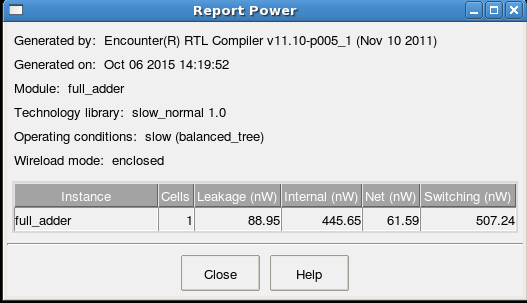
\includegraphics[width=0.7\textwidth]{images/power.png}
\caption{Power Consumed by Full Adder}
\end{figure}

\subsubsection*{Layout}
\FloatBarrier
\begin{figure}[!htpb]
\centering
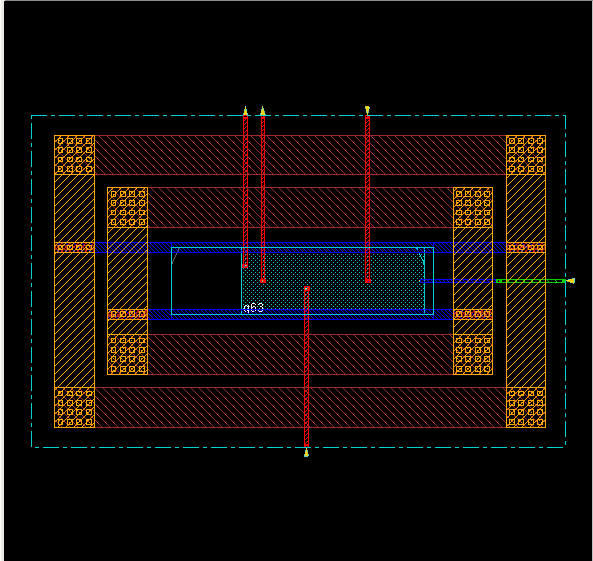
\includegraphics[width=0.8\textwidth]{images/layout.png}
\caption{Layout of Full Adder}
\end{figure}

\subsubsection*{Area Consumed in Layout}
\FloatBarrier
\begin{figure}[!htpb]
\centering
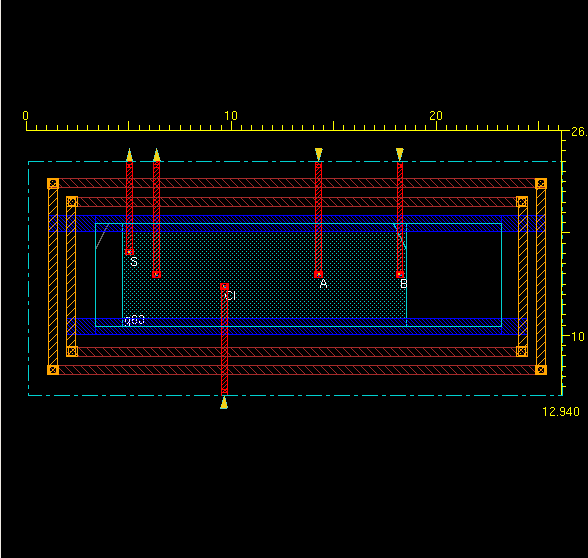
\includegraphics[width=0.8\textwidth]{images/layoutarea.png}
\caption{Area Consumed by Full Adder in Layout}
\end{figure}

\subsubsection*{Gate Level Simulation}
\FloatBarrier
\begin{figure}[!htpb]
\centering
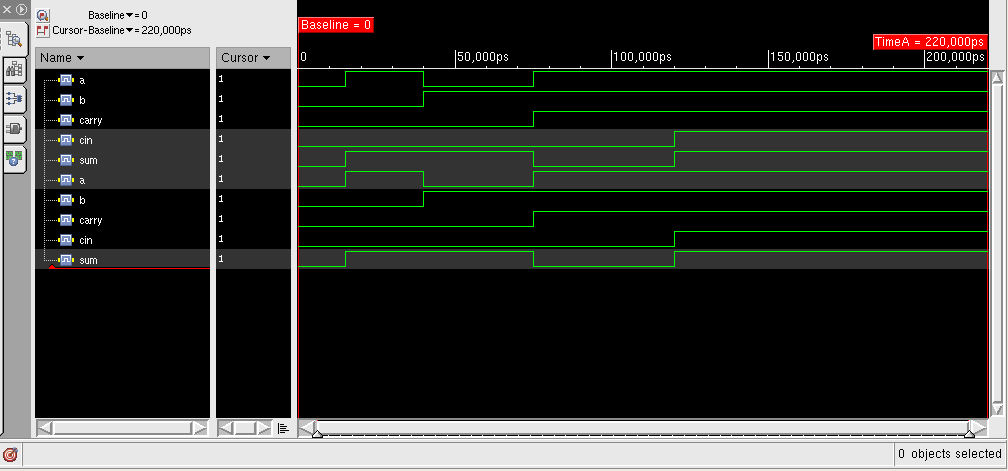
\includegraphics[width=0.9\textwidth]{images/gatelevel1.png}
\caption{Gate Level Simulation of Full Adder}
\end{figure}



\subsection*{Result}

Designed and synthesized  a full adder using  verilog and verified its functionality using RTL and Gate Level Simulation and also drawn its layout.  The area, power and delay of full adder is found out.



\subsection{Project Organization}
	The project is split-up into 6 stages as shown in table :\\
	
\begin{tabular}{|c|c|c|}\hline
Sl No&Work& Duration(in Weeks)\\ \hline \normalsize
1&Information Collection on DFB \& VNC&1 \\ \hline
2&Information collection on development tools&2\\ \hline
3&Integrating DirectFB \& VNC&8\\ \hline
4&Cross Compiling \& Porting&2\\ \hline
5&Building JPEG libraries&2\\ \hline
6&Testing&2\\ \hline
\end{tabular}


